\documentclass{bioinfo}
\copyrightyear{xxx} \pubyear{xxx}

\access{Advance Access Publication Date: Day Month Year}
\appnotes{Manuscript Category}

\usepackage{algorithm}
\usepackage{algpseudocode}
\usepackage{subfigure}
\renewcommand{\algorithmicrequire}{\textbf{Input:}}
\renewcommand{\algorithmicensure}{\textbf{Output:}}

\renewcommand\qedsymbol{$\blacksquare$}
\theoremstyle{definition}
\newtheorem{thm}{\textbf{Theorem}}[section]%
\newtheorem{cor}{\textbf{Corollary}}[thm]%
\newtheorem{lem}[thm]{\textbf{Lemma}}%
\newtheorem{defn}{\textbf{Definition}}[section]%

\begin{document}
\firstpage{1}

\subtitle{Subject Section}

\title[SGOPT]{SGOPT:Alignment of dynamic protein-protein interaction networks based on segment tree optimization}
\author[Sample \textit{et~al}.]{Corresponding Author\,$^{\text{\sfb 1,}*}$, Co-Author\,$^{\text{\sfb 2}}$ and Co-Author\,$^{\text{\sfb 2,}*}$}
\address{$^{\text{\sf 1}}$Department, Institution, City, Post Code, Country and \\
$^{\text{\sf 2}}$Department, Institution, City, Post Code,
Country.}

\corresp{$^\ast$To whom correspondence should be addressed.}

\history{Received on XXXXX; revised on XXXXX; accepted on XXXXX}

\editor{Associate Editor: XXXXXXX}

\abstract{\textbf{Motivation:} The alignment of protein-protein interaction (PPI) networks makes us better understanding biological relationships between different species. For now, many different network alignment methods have been proposed, but they can only be used to align static PPI networks. However, biological systems are always dynamic. Model PPI networks as dynamic networks is more suitable for the purpose of understanding the life process of biological systems. Thus, a new alignment method for dynamic networks is strongly needed in this situation.\\
\textbf{Results:} In this work, we focus on the alignment of one static PPI network and one dynamic PPI network. To solve this problem, we propose a novel alignment method called SGOPT (SeGment tree OPTimization). SGOPT can be used based on any state-of-the-art static network alignment methods and is a general framework to transform static alignments to dynamic alignments with a higher alignment quality. Through systematical evaluation on real-world PPI data, we demonstrate that SGOPT is very efficient to produce good dynamic alignments of PPI networks.\\
\textbf{Availability:}xxxxx\\
\textbf{Contact:} \href{name@bio.com}{name@bio.com}\\
\textbf{Supplementary information:} Supplementary data are available at \textit{Bioinformatics}
online.}

\maketitle
%@@@@@@@@@@@@@@@@@@@@@@@@@@@@@@@@@@@@@@@@@@@@@@@@@@@@@@@
\section{Introduction}

Protein-protein interaction (PPI) networks are used to model proteins and their interactions in different species. By analyzing PPI networks, we can discover many biological knowledge about how cell works. Also, through the alignment of PPI networks for different species, we get biological knowledge transferred from one species to the other one. 

Network alignment (NA) aims to find highly conserved regions among PPI networks. NA will generate a node mapping from one PPI network to the other PPI network. According to different purposes, NA can be local (LNA) or global (GNA), and the node mapping can be one-to-one or many-to-many. 

For the LNA, the purpose is to find very similar regions between PPI networks. Usually the regions are very small such as a pathway or a motif, and one region in a network may be aligned to more than one regions in the other network leading to a many-to-many node mapping. Alignment methods for LNA includes PathBLAST\citep{kelley2004pathblast}, NetworkBLAST\citep{sharan2005conserved}, NetAlign\citep{liang2006netalign}, MaWISh\citep{koyuturk2006pairwise} and so on.

For the GNA, usually it aims to find an overall node mapping from one network to another \citep{singh2008global,liao2009isorankn,kuchaiev2011integrative,malod2015graal,kuchaiev2010topological,memivsevic2012c,saraph2014magna,vijayan2015magna++,aladaug2013spinal,kazemi2016proper}. In GNA, one node from the source network is aligned to only one node in the target network. Thus, GNA will generates a global one-to-one node mapping. In this paper, we focus on GNA problem.

However, all these NA (LNA or GNA) methods, they are all static alignment methods which means that they can only be used to align static PPI networks. But during the whole life process of a cellular system, the interactions between proteins will change over time. Although static PPI networks can model PPIs, they can not capture the temporal information of PPIs. There are some works that demonstrate how we can build a dynamic PPI network based on gene expression data or other biological information.\citep{chen2014identifying,wang2013construction,zhang2016method}. 

Based on these works, could we generate an alignment of dynamic PPI networks and measure the quality of the alignment? To our knowledge, there are few works which handle this problem.

This paper introduces the alignment problem of one static PPI network and one dynamic PPI network. Also, SGOPT (SeGment tree OPTimization), a general framework is proposed which can transform any static alignments to dynamic alignments with a higher alignment quality. SGOPT uses a local optimization strategy to adjust initial static alignments iteratively and produce dynamic alignments based on a data structure called segment tree. Through experiment evaluations, SGOPT shows the potentiality that it can produce good dynamic alignments in a time-saving manner.

%\enlargethispage{12pt}

\begin{methods}
%@@@@@@@@@@@@@@@@@@@@@@@@@@@@@@@@@@@@@@@@@@@@@@@@@@@@@@@@@@@@@@@@@
\section{Methods}
Because there are few works describing the concept of dynamic alignments, first we should give the definition of dynamic alignments, along with new alignment quality measurements. Then, we propose two naive ways that apply state-of-the-art static alignment methods to produce dynamic alignments. The two ways will be compared with our SGOPT methods in experiments. At last, we give the details about our main contribution in this paper, the SGOPT framework.
%@@@@@@@@@@@@@@@@@@@@@@@@@@@@@@@@@@@@@@@@@@@@@@@@@@@@@@@@@@@@@@@@@
\subsection{Problem definition}
\begin{defn}[Dynamic PPI network]
\label{defndppi}
Let $G=(V,E)$ be a \textit{dynamic PPI network}. $V$ denotes the node set of proteins and $E$ denotes the edge set of \textit{dynamic} protein-protein interactions. For every edge $e\in E, e$ has the form $(u_e,v_e,l_e,r_e)$ which means that the interaction between proteins $u_e$ and $v_e$ exists from time $l_e$ to $r_e$. Here, the time is discrete and start from 1. Let $T_G=max\{r_e: e\in E\}$ denotes the maximum value of the time across all the dynamic protein-protein interactions.
\end{defn}

From the definition \ref{defndppi}, we can see that the difference between a dynamic PPI network and a static PPI network is whether a PPI has an time interval in which it's active. So for the static network, the edge $e$ has the form $(u_e,v_e)$.

\begin{defn}[Instance network]
\label{defninstance}
In general, a dynamic PPI network $G(V,E)$ can be treated as combination of $T_G$ static PPI networks. At time $i$, we call the static PPI network $G_i=(V,E_i)$ an \textit{instance network} of $G$. $E_i=\{(u_e,v_e):e\in E,l_e\leq i\leq r_e\}$ denotes the edge set of $G_i$.
\end{defn}

According to the definition \ref{defndppi} and \ref{defninstance}, a dynamic PPI network is made up of many static PPI networks, and at different times, the dynamic network can be seen as different static networks. That is what \textit{dynamic} means.

\begin{defn}[Dynamic alignment]
\label{defndppigna}
Let $SG=(SV,SE)$ be a static PPI network and $DG=(DV,DE)$ be a dynamic PPI network (without loss of generality, $|SV|\leq |DV|$). A \textit{dynamic alignment} of these two PPI networks is a one-one node mapping $f:SV\rightarrow DV,\forall v_1,v_2\in SV,f(v_1)\neq f(v_2)$. 
\end{defn}

We can see that the alignment of dynamic PPI networks is similar to the static version except the target network is a dynamic PPI network. For one node $v_1\in SV$, if $v_1$ is mapped to some node $v_2\in DV$ ($f(v_1)=v_2$), we say that $(v_1,v_2)$ is an \textit{alignment pair} and $v_2$ is the \textit{aligned node} of $v_1$ beyond alignment $f$, vice versa. Otherwise, we say $v_1$ is not aligned. Also, there will be no two nodes aligned to the same node.

For convenience, we use the word \textit{dynamic alignment} when we consider the alignment of dynamic PPI networks, \textit{static alignment} when there comes the static case.

\begin{defn}[Conserved edge, mapping edge]
\label{defnceme}
Let $f$ be an alignment of a static network $SG$ and a dynamic network $DG$. For one edge $(u,v)\in SE$, if $(f(u),f(v))\in DE_i$, we say $(u,v)$ is a \textit{conserved edge} and $(f(u),f(v))$ is a \textit{mapping edge} at time $i$. 
\end{defn}

According to the definition \ref{defnceme}, $f_i(SE)=\{(u,v):(u,v)\in SE,(f(u),f(v))\in DE_i\}$ is a set which consists of all conserved edges at time $i$. 

As we know, for static alignments, there are many alignment quality measurements defined to tell whether an alignment is good or bad. So, like the static measurements, we define new alignment quality measurements for the dynamic alignments based on the static alignment quality measurement.
\begin{defn}[Dynamic alignment quality measurements]
\label{defndmeasure}
Let $f$ be an alignment of a static network $SG$ and a dynamic network $DG$. Define $$DEC(f)=\underset{i}{max}\frac{\left | f_i(SE) \right |}{\left | SE \right |}$$ be the \textit{DEC} measurement of dynamic alignment $f$, it calculates the maximum ratio of number of the conserved edges to the number of edges in $SG$ across all the times.
Similarly, 
$$DICS(f)=\underset{i}{max}\frac{\left | f_i(SE) \right |}{\left |DE_i(DG[f(SV)])\right |}$$ is the \textit{DICS} measurement which calculates the maximum ratio of the number of conserved edges to the number of edges in the subgraph of $DG_i$ which is induced by the aligned node set under alignment $f$ across all the times,
$$DS^{3}(f)=\underset{i}{max}\frac{\left | f_i(SE) \right |}{\left | SE \right |+\left |DE_i(DG[f(SV)]) \right |-\left | f_i(SE) \right |}$$ is the \textit{DS}$^{3}$ measurement which calculates the maximum ratio of number of the conserved edges to the number of edges which is an union set of $SE$ and mapping edges in $DE_i$ across all the times,
$$DTWEC(f)=\underset{i}{max}(\frac{\left | f_i(SE) \right |}{\left | SE \right |}+\frac{\left | f_i(SE) \right |}{\left |DE_i(DG[f(SV)])\right |})/2$$ is the \textit{DTWEC} measurement which is an average estimate about $DEC$ and $DICS$ measurements. 

Here, $f(SV)=\{f(u)\in DV:u\in SV\}$ is a set which consists of all aligned nodes in $DG$ and $DG[X]$ is the induced subgraph of $DG$ by node set $X$.
\end{defn}

The definition \ref{defndmeasure} gives us some quality measurements for any dynamic alignments. We can see that all the dynamic-version measurements are actually the extension of the corresponding static-version measurements which calculates the maximum value of static-version measurements across all the times.

\textbf{Dynamic PPI network alignment problem}. We define the problem as that of finding a dynamic alignment which can maximize the corresponding dynamic alignment quality measurement. Formally, we want to find a dynamic alignment $f$ such that $Q(f)$ is as large as possible, where $Q(f)$ is some dynamic alignment quality measurement for $f$.

\textbf{The CE measurement}. The alignment quality measurements give us a hint that a good alignment is alway an alignment that has a large number of conserved edges. That's also the motivation of our method. Actually in this work, what we expected to do, is to maximize the CE measurement of a dynamic alignment. Here, we give its formal definition.

\begin{defn}[CE measurement]
\label{defnce}
Let $f$ be an alignment of a static network $SG$ and a dynamic network $DG$, define the \textit{CE (conserved edge) measurement} of $f$ as 
$$CE(f)=\underset{i}{max}\{ |f_i(SE)|\}$$
\end{defn}

%@@@@@@@@@@@@@@@@@@@@@@@@@@@@@@@@@@@@@@@@@@@@@@@
\subsection{Application of state-of-the-art static methods}
For now, there already have many alignment methods that aim to find global alignments of PPI networks, but they are all used for static PPI networks and can not be used in our dynamic case directly. Nevertheless, we propose two naive ways to apply state-of-the-art static alignment methods to produce dynamic alignments.

\textbf{Case 1}. Let $SG$ be the static network and $DG$ be the dynamic network. For the first case, we just ignore the $l_e,r_e$ for every edge $e\in DE$ and treat it as a static PPI network $DG(DV,DE)$. Then we apply any state-of-the-art static methods to align $SG$ and $DG$. Finally, we use the alignment generated by the static method as our dynamic alignment.

\textbf{Case 2}. For the second case, consider all the instance networks $DG_i$ of $DG$. What we should do, is to use static methods to align every pair of networks $SG$ and $DG_i$. At last we will get several static alignments and we pick the one with the highest alignment quality measurement as our dynamic alignment.

The two ways of applying state-of-the-art methods in our problem are very simple and have their own advantages and disadvantages. For the first case, we just need to align networks once but maybe produce a bad alignment. For the second case, we need to align networks $T_{DG}$ times to get a good alignment which is too time consuming if $T_{DG}$ is very large.

%@@@@@@@@@@@@@@@@@@@@@@@@@@@@@@@@@@@@@@@@@@@@@@@@@@
\subsection{The SGOPT alignment method}
According to the definition \ref{defnce}, what we seek is the maximum number of conserved edges between $SG$ and all instance networks $DG_i$ for the alignment $f$. Thus, what SGOPT does, is to find a dynamic alignment $f$ that maximize $CE(f)$.
%@@@@@@@@@@@@@@@@@@@@@@@@@@@@@@@@@@@@@@@@@@@@@@@@@@@@@
\subsubsection{General framework}
The SGOPT method is actually a general framework which can be used to improve any alignments produced by static alignment methods, so the input of the SGOPT method can be any alignments. 

The SGOPT method is consist of two main parts, the local optimization strategy part and the segment tree optimization part. The main idea of SGOPT is to use a local optimization strategy to improve any alignments iteratively in terms of the CE measurement. And for increasing the speed of calculating the CE measurements, a data structure called segment tree is used to guarantee the efficiency.

%@@@@@@@@@@@@@@@@@@@@@@@@@@@@@@@@@@@@@@@@@@@@@
\subsubsection{The local optimization strategy}
SGOPT uses a local optimization strategy to adjust any initial alignment $f$ iteratively and make $CE(f)$ as large as possible.

\begin{defn}[Adjustment of the alignment]
\label{defnadj}
Let $f$ be an alignment of one static network $SG$ and one dynamic network $DG$. Let $(x,y)$ be a pair that $x\in SV,y\in DV$. There are two cases at which we call the pair $(x,y)$ an \textit{adjustment} of the alignment $f$. For the first case, neither $x$ nor $y$ is aligned and we make $(x,y)$ a new alignment pair for $f$. For the second case, $(x,y)$ is already an alignment pair of $f$, and we remove this alignment pair from $f$, making $x$ and $y$ unaligned.
\end{defn}

\begin{defn}[Pair contribution]
\label{defncontribute}
Let $f$ be an alignment of one static network $SG$ and one dynamic network $DG$. For one pair $(x,y),x\in SV,y\in DV$ that $x$ and $y$ are not aligned, define the \textit{pair contribution} of $(x,y)$ for $f$ as $$C_f(x,y)=|\{(u,v):u\in N(x),v\in N(y),f(u)=v\}|$$. Here, $N(x)$ denotes the set of nodes which are neighbors of node $x$.
\end{defn}

We can see that the pair contribution is an estimate of added conserved edges if this pair is aligned.

\textbf{General process and the algorithm}. The main idea of the strategy is to make lots of adjustments of the alignment $f$ iteratively based on a local optimization model. In each iteration, we pick some alignment pairs of $f$ randomly and remove these pairs from $f$. Then we construct a weighted bipartite graph $bg$ whose two partitions are consist of unaligned nodes in $SV$ and $DV$ respectively. Every edge in $bg$ is weighted by its pair contribution. A maximum weighted bipartite graph matching is produced by some bipartite graph matching algorithm. For every match of the graph matching, it stands for a new alignment pair which we will add to the alignment $f$.

See Algorithm~\ref{alg:1} for more details. As we can see from the algorithm, it is an iterative algorithm and for an iterative algorithm we should setup a number of total iterations the algorithm will run for, that is what $\alpha$ means. For $\beta$, it stands for the number of alignment pairs we will remove in each iteration. 

For $\alpha$, if it is too large, the algorithm will be time consuming. On the other side, if it is too small, the algorithm may not produced good alignments. We should see how $\alpha$ effects the algorithm.

For $\beta$, if it is too large, there will be a large bipartite graph constructed in each iteration and it will take more time in each iteration. Also, $\beta$ is an important factor that may influence the chance of finding a better alignment in each iteration.Thus, we should see how $\beta$ effects the algorithm.
\begin{algorithm}[!tpb]
    {
    \caption{The SGOPT algorithm}
    \label{alg:1}
        \begin{algorithmic}[1]
        \Require
        $SG(SV,SE)$: the static network
        
        $DG(DV,DE)$: the dynamic network 
        
        $f$: the initial alignment need to adjust
        
        $\alpha$: the parameter of the SGOPT algorithm, denotes the number of total iterations the algorithm will run
        
        $\beta$: the parameter of the SGOPT algorithm, denotes the number of alignment pairs the algorithm will remove in each iteration
        
        \Ensure
        $f$: the final alignment after adjustment
        
        \State calculate $CE(f)$
        \State $iteration\_count \gets 0$
        \While{$iteration\_count<\alpha$}
            \State $iteration\_count\gets iteration\_count+1$
            \State $oldf\gets f$
            \State $ds\gets$ a randomly picked set of alignment pairs for $f$ whose size is determined by $\beta$
            \State $\forall (x,y)\in ds$, make adjustment of $f$ using $(x,y)$.
            \State $bg\gets WeightedBipartiteGraph(SV/f,DV/f,C_f(x,y))$
            \State $M\gets MaximumWeightedBipartiteGraphMaching(bg)$
            \State $\forall (x,y)\in M$, make adjustment of $f$ using $(x,y)$
            \State re-calculate $CE(f)$
            \If{$CE(f)<CE(oldf)$}
                \State $f\gets oldf$
            \EndIf
        \EndWhile
        \end{algorithmic}    
    }
    \end{algorithm}
\end{methods}

%@@@@@@@@@@@@@@@@@@@@@@@@@@@@@@@@@@@@
\subsubsection{The segment tree optimization}
According to the algorithm~\ref{alg:1}, in each iteration, we shall maintain $CE(f)$ while a new candidate alignment $f$ is being constructed. In this work, we introduce an optimization framework to maintain $CE(f)$ very efficiently. The main idea of the optimization framework is a data structure called segment tree.

\textbf{Segment tree}. Segment tree is a data structure which is very suitable to solve sequence problems. In general, a segment tree is a binary tree whose nodes stands for a interval of the sequence. The root of the binary tree stands for the whole sequence. For a node in the binary tree, if the length of interval is not 1, then it will have two child nodes whose length is half of the length of the interval of the parent node. As a result, for a sequence with length $T$, a segment tree with a height no more than $log(T)$ can be constructed. It can be proved that any interval operations can be done in $O(log(T))$ in the segment tree.

Because what we care about is the speed of calculating $CE(f)$, so we should see what the time complexity is whether we use a segment tree or not.

\textbf{Maintain $CE(f)$ without a segment tree}. If we directly maintain $CE(f)$ without a segment tree, the time complexity of maintaining $CE(F)$ is $O(T_{DG})$, see Theorem~\ref{thmsingleforce} and Corollary~\ref{corsingleforce} for details.
\begin{thm}
\label{thmsingleforce}
Let $f$ be the alignment of one static network $SG$ and one dynamic network $DG$. The time complexity to calculate $CE(f)$ is $O(|SE|*T_{DG})$
\end{thm}
\begin{proof}
For the purpose of calculating $CE(f)$, basically we should calculate all $f_i(SE)$ at every time $i$ and pick the one with largest set size. For the purpose of calculating $f_i(SE)$, we should check every edge in $SE$ to see if it's a conserved edge at time $i$ which can be done in $O(1)$. Thus, it takes $O(|SE|)$ to calculate $f_i(SE)$ for a fixed time and $O(|SE|*T_{DG})$ to calculate all sets over time. 
\end{proof}
\begin{cor}
\label{corsingleforce}
Let $f$ be the alignment of one static network $SG$ and one dynamic network $DG$. If $f$ is changed and makes only one edge $(u,v)\in SE$ change its mapping (the aligned node of either of its two nodes), the time complexity to re-calculate $CE(f)$ is $O(T_{DG})$. 
\end{cor}
\begin{proof}
Because only the mapping of the edge $(u,v)\in SE$ is changed, just re-check $(u,v)$ to see if it's conserved at every time $i$ and renew the corresponding set $f_i(SE)$.
\end{proof}


\textbf{Reduce the time complexity from $O(T_{DG})$ to $O(log(T_{DG}))$}. The corollary \ref{corsingleforce} shows that if one edge in $SE$ changes its' mapping, we should check its' state at every time. But actually the time complexity can be reduce to $O(log(T_{DG}))$ is a segment tree is used, see Theorem~\ref{thmsingletree} for details.

\begin{thm}
\label{thmsingletree}
For the problem in corollary \ref{corsingleforce}, it takes $O(log(T_{DG}))$ to renew $CE(f)$ if a segment tree is used.
\end{thm}
\begin{proof}
Let $x_1$ be the aligned node of $u$ and $y_1$ be the aligned node of $v$ before $f$ is changed. Let $x_2$ be the aligned node of $u$ and $y_2$ be the aligned node of $v$ after $f$ is changed.

For the first case, $(x_1,y_1)$ is not an mapping edge of $DE$ at any time which means that $(u,v)$ is not a conserved edge at any time. Thus, the set size of $f_i(SE)$ will not change for every $i$ if we remove the mapping of $(u,v)$.

For the second case, $(x_1,y_1)=(u_e,v_e)$ for some edge $e\in DE$ which means that $(u,v)$ is a conserved edge from time $l_e$ to $r_e$. Thus, the set size of $f_i(SE)$ will decrease by one in this time interval if we remove the mapping of $(u,v)$.

The two cases can also be applied to $(x_2,y_2)$ if we add the new mapping of $(u,v)$. And we can conclude that every time a mapping of one edge changes, some values of $|f_i(SE)|$ in a time interval will increase by one and some values of $|f_i(SE)|$ will decrease by one. If we treat all values of $|f_i(SE)|$ as an integer sequence, then every time we will increase or decrease all the values by one in some interval.As for the calculation of $CE(f)$, we just need to know the largest value of the integer sequence.

As all the changes of an integer sequence can be maintained by the segment tree data structure in $O(log(T_{DG}))$, the time complexity of re-calculation of $CE(f)$ can be reduced to $O(log(T_{DG}))$.
\end{proof}

\begin{cor}
\label{corntree}
Let $f$ be the alignment of one static network $SG$ and one dynamic network $DG$. If $f$ is changed and makes $N$ edges $(u,v)\in SE$ change their mappings, the time complexity of re-calculate $CE(f)$ is $O(N*log(T_{DG}))$. 
\end{cor}

%@@@@@@@@@@@@@@@@@@@@@@@@@@@@@@@@@@@@@@@@@@@@@@@@@@@@@@@@@@@
\subsubsection{Time complexity analysis} 

According to the definition \ref{defnadj}, if we make an adjustment $(u,v)$ of the alignment $f$. There will be $|N(u)|$ edges whose mapping will be changed. Thus it takes $O(|N(u)|*log(T_{DG}))$ to re-calculate the $CE(f)$ (corollary \ref{corntree}).

The main running time of the algorithm is consumed on the iterations. In each iteration, it takes $O(\beta)$ to pick the alignment pairs which need to be removed from $f$. And for every alignment pair $(u,v)$, it takes $O(|N(u)|*log(T_{DG}))$ to remove it. Because we choose the alignment pairs randomly, so the value of $|N(u)|$ can be approximately estimated by $Avg(SG)$ which is the average node degree of $SG$. So it takes $O(\beta*Avg(SG)*log(T_{DG}))$ to complete the adjustment of the alignment $f$ in every iteration.

For the construction of the bipartite graph, there will be at most $O(\beta)$ nodes in one partition of the bipartite graph. So it takes $O(\beta^2*Avg(DG)*Avg(SG))$ to construct the bipartite graph. In our experimental implementation we use a greedy strategy to construct the maximum weighted matching which only takes $O(\beta^2)$.

So the overall time complexity is $O(\alpha*(\beta^2*Avg(DG)*Avg(SG)+\beta*Avg(SG)*log(T_{DG})))$.


%@@@@@@@@@@@@@@@@@@@@@@@@@@@@@@@@@@@@@@@@@@@@@@@@@@@@@@@@@@@@@@
\section{Results and discussion}
%@@@@@@@@@@@@@@@@@@@@@@@@@@@@@@@@@@@@@@@@@@@@@@@@@@@@@@@@@@@
\subsection{Data collecting and preprocessing}
We experiment the SGOPT method on real-world PPI data. All PPI data are collected from IsoBase \citep{park2011isobase} which is a commonly used PPI data database. We pick the PPI data for four species:\textit{Saccharomyces cerevisiae}, \textit{Drosophila melanogaster}, \textit{Caenorhabditis elegans} and \textit{Homo sapiens}. Since all the PPI networks collected from IsoBase are static networks, we use the three-sigma method\citep{zhang2016construction} to construct the corresponding dynamic networks. As a result, we get four dynamic PPI networks for every species.

Because in this paper, the problem is for one static network and one dynamic network, we wish the static network is chosen as an instance network of the corresponding dynamic network. Therefore, we pick out one instance network of the dynamic network and use it as our static network for the experiments. Please see Table.~\ref{table:1} and Table.~\ref{table:2} for more details about the experimental data.

\begin{table}[!h]
\processtable{Details of four static PPI networks\label{table:1}}
{
\begin{tabular}{@{}llll@{}}
\toprule 
Species & Proteins & Interactions & Average node degree\\
\midrule
C.elegans & 2974 & 2653 & 1.78\\
D.melanogaster & 7387 & 14004 & 3.79\\
H.sapiens & 10296 & 30349 & 5.90\\
S.cerevisiae & 5523 & 46207 & 16.73\\
\botrule
\end{tabular}
}{}
\end{table}


%@@@@@@@@@@@@@@@@@@@@@@@@@@@@@@@@@@@@@@@@@@@@@@@@@@@@@@@@
\subsection{Methods and metrics}
SGOPT is implemented in Java and the software is available as part of the Supplementary Material. All experiments are performed on a 64-bit machine with Intel Core i7 4.00GHz processors and 16 GB of memory. 

In this paper, we compare SGOPT with four methods.The first method is IsoRank\citep{singh2008global}. IsoRank is the first GNA method which aims to align two PPI networks globally, it defines \textit{node similarity} between the two PPI networks based on protein-protein BLAST scores\citep{altschul1990basic} and topological similarity. It uses a factor $\alpha$ to control the balance between the two kinds of scores. IsoRank will produce the final alignment using a greedy or optimal algorithm after the node similarity is calculated .

The L-GRAAL\citep{malod2015graal} method is the most recent work of the GRAAL family. It models the alignment problem as an \textit{integer programming} problem and produce the final alignment by solving the problem with Lagrangian relaxation.

\begin{table}[!h]
\processtable{Details of four dynamic PPI networks. Average interactions measure the average number of edges among all the $T_{DG}$ instance networks\label{table:2}}
{
\begin{tabular}{@{}llll@{}}
\toprule 
Species & $T_{DG}$ & Proteins & Average interactions\\
\midrule
C.elegans & 15 & 2974 & 1896.87\\
D.melanogaster & 15 & 7387 & 9995.27\\
H.sapiens & 15 & 10296 & 21772.73\\
S.cerevisiae & 15 & 5523 & 32990.53\\
\botrule
\end{tabular}
}{}
\end{table}

The SPINAL\citep{aladaug2013spinal} method is a two-phase method. In the first phase, SPINAL computes a confident score between every pair of nodes of two PPI networks based on node similarity and topological similarity. In the second phase, an alignment is iteratively produced by a seed-and-extend strategy.

The PROPER\citep{kazemi2016proper} method uses BLAST scores as the node similarity between PPI networks and produces a \textit{seed set} of the alignment by choosing the alignment pairs whose BLAST scores are larger some threshold. Based on the seed set, PROPER iteratively adds new alignment pairs to the seed set based on the pair contributions.

For every method we compared with, we apply it to produce dynamic alignments with two ways, as we said, these are two simple ways. The third way is to use our framework SGOPT based on the alignments generated by static methods. For every experiment that aligning two PPI networks, we will compare alignment results produced in all three ways.

We use the CE measurement and running time as our experimental metrics because they are main factors of the SGOPT algorithm. Also, we will compare SGOPT with four methods using other measurements.

We use \textit{Method-W1, Method-W2} to denote the alignment results produced by \textit{Method} in two ways. For example, \textit{IsoRank-W1} denotes the alignment results produced by the IsoRank method using the first way. And we use \textit{SGOPT-Method} to denote the alignment results produced by SGOPT based on \textit{Method-W1} alignment results.

%@@@@@@@@@@@@@@@@@@@@@@@@@@@@@@@@@@@@@@@@@@@@@@@@@@@@@@@@@@@@
\subsection{The effect of parameters $\alpha$ and $\beta$}
\textbf{The effect of $\mathbf{\beta}$}. As we can see from the SGOPT algorithm, $\beta$ controls the number of alignment pairs to be removed from $f$ in each iteration. For different $\beta$, we want to see how it effects the the experimental results. 

Fig.~\ref{beta} shows the results. Specifically, Fig.~\ref{beta1} is the experimental results when we test for big $\beta$ with a big step value. We observe that, with a fixed $\beta$, the CE measurement of the alignment with a long running time is better than that with a short running time, which is what we expected. Second, for the same running time, we find that the smaller the $\beta$ is, the better the CE measurement of the alignment is. With large $\beta$ like 600, it can not even improve the initial alignment produced by SPINAL-W1 in 300 seconds. We guess that it's because the more pairs we removed, the more difficult we can adjust the current alignment to a better one. Therefore, small $\beta$ is preferred for SGOPT. In fact, with small $\beta$, SGOPT can adjust the alignment in a local manner and produced a better alignment faster than that in a global manner.

We also test for small $\beta$ with a small step value. Fig.~\ref{beta2} shows that with small $\beta$, there is no obvious gap between different $\beta$. Thus, we guess that SGOPT is more suitable for small $\beta$ and we use $\beta=35$ as our default parameter for next experiments.

\begin{figure}[!htbp]
    \subfigure[$\beta$ from 50 to 2000 with a step value of 50]{
        \begin{minipage}[b]{\linewidth}
            \centering
            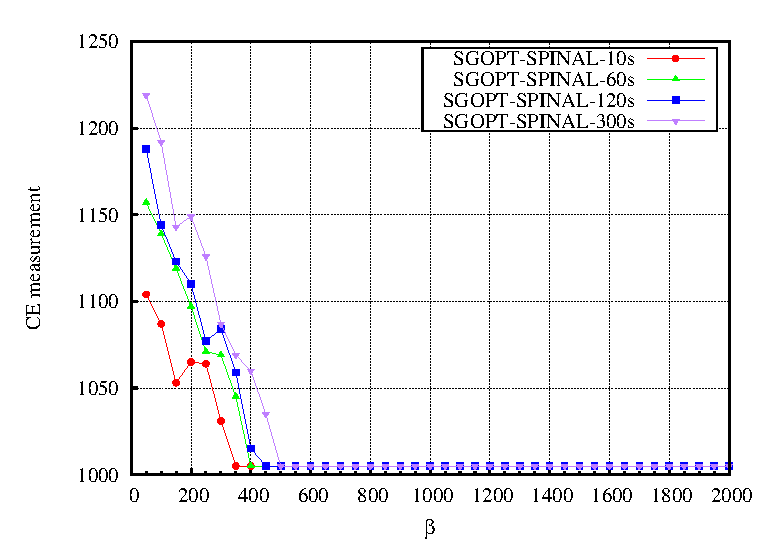
\includegraphics[width=\linewidth]{pic/beta1.eps}
            \label{beta1}
        \end{minipage}
    }
   \subfigure[$\beta$ from 5 to 50 with a step value of 3]{
        \begin{minipage}[b]{\linewidth}
            \centering
            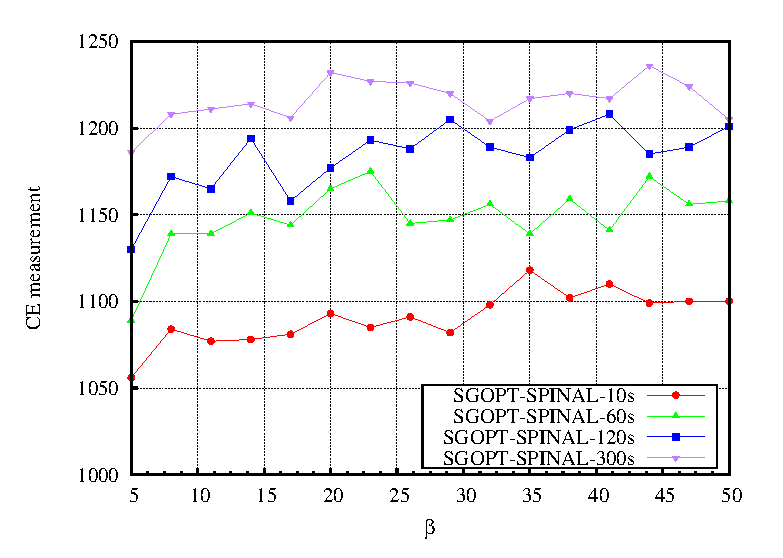
\includegraphics[width=\linewidth]{pic/beta2.eps}
            \label{beta2}
        \end{minipage}
    }
    \caption{The effect of the $\beta$ parameter while running SGOPT-SPINAL aligning C.elegans and D.melanogaster PPI networks, different lines stand for different running time. }
    \label{beta}
\end{figure}

\textbf{The effect of $\mathbf{\alpha}$}. Since $\alpha$ controls the total number of iterations, we shall see how the CE measurement changes after every iteration. Fig.~\ref{alpha} shows the experimental results. Specifically, from Fig.~\ref{alpha1} we observe that the CE measurement will become better after every iteration.

Fig.~\ref{alpha2} shows the difference of CE measurements between continuous iterations. We find that, the chance of getting better CE measurements gets fewer over iterations which means that SGOPT will converge eventually. In general, the larger number of iterations is preferred. But considering the running, we pick $\alpha=15000$ as our default parameter for next experiments.

\begin{figure}[!htbp]
    \subfigure[CE measurement]{
        \begin{minipage}[b]{\linewidth}
            \centering
            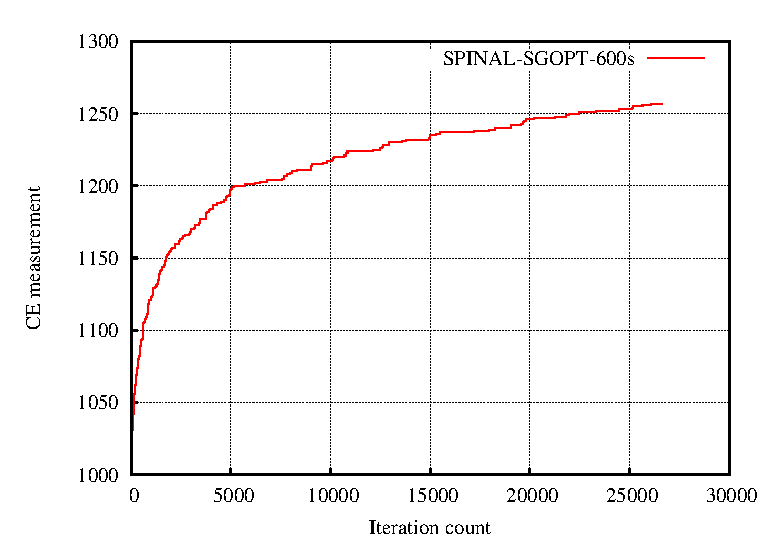
\includegraphics[width=\linewidth]{pic/alpha.eps}
            \label{alpha1}
        \end{minipage}
    }
   \subfigure[CE measurement(difference)]{
        \begin{minipage}[b]{\linewidth}
            \centering
            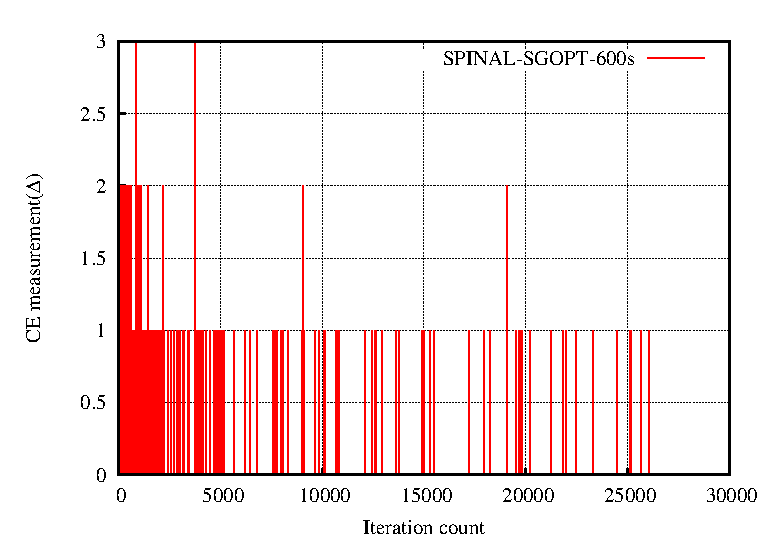
\includegraphics[width=\linewidth]{pic/alphad.eps}
            \label{alpha2}
        \end{minipage}
    }
    \caption{The effect of the $\beta$ parameter while running SGOPT-SPINAL aligning C.elegans and D.melanogaster PPI networks. }
    \label{alpha}
\end{figure}
%@@@@@@@@@@@@@@@@@@@@@@@@@@@@@@@@@@@@@@@@@@@@@@@@@@@@@@@@@@@@
\subsection{Comparison using different methods}
As every method has their own parameters, in this paper, we will use the default values of parameters for all the four methods.

\textbf{The CE measurement and running time}. Fig.~\ref{ce-dm} shows the CE measurement and running time while we experiment four methods in three ways aligning C.elegans and D.melanogaster PPI networks. For the results of aligning other PPI networks, see Supplementary Figs S1-S5. 

For the CE measurement, in general, \textit{SGOPT-Method} always has better alignments than \textit{Method-W1} for every method, which are still worse than alignments produced by \textit{Method-W2}. The exception is that \textit{SGOPT-IsoRank} has much more better alignments than both \textit{IsoRank-W1} and \textit{IsoRank-W2}. And in the Supplementary Fig S5(a), we observe that \textit{SGOPT-SPINAL} has better alignments than \textit{SPINAL-W2}.

For the running time, we find that \textit{Method-W2} is very time consuming even though it can produce good alignments. That's where the advantage of SGOPT is. Compared to \textit{Method-W1}, SGOPT can produce better results within an acceptable running time. Compared to \textit{Method-W2}, SGOPT can save a large running time, although having a worse alignment.  

There is an exception for the PROPER method. From all the results, we observe that even in \textit{PROPER-W2}, the algnment result is better than SGOPT from the aspect of either CE measurement or running time. But SGOPT has a potential advantage if the number of time of the dynamic PPI network increases. PROPER is better at saving time than SGOPT for $T_{DG}=15$, but will fail with larger value of $T_{DG}$ because the time complexity of \textit{PROPER-W2} is proportional to $O(T_{DG})$, but for SGOPT, this is $O(log(T_{DG}))$.

Therefore, for the trade-off between the CE measurement and running time, we conclude that SGOPT could be a method which can produce good alignments in short time.
\begin{figure}[!htbp]
    \subfigure[CE measurement]{
        \begin{minipage}[b]{\linewidth}
            \centering
            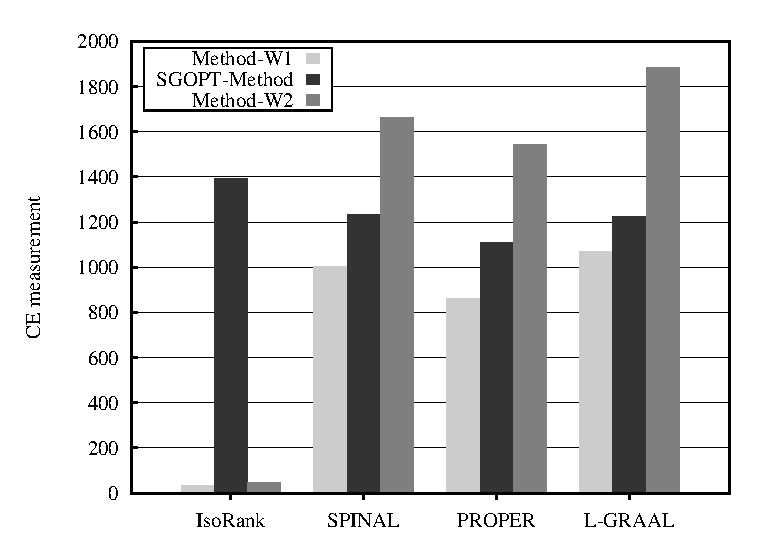
\includegraphics[width=\linewidth]{pic/ce-dm-CE.eps}
            \label{ce-dm-CE}
        \end{minipage}
    }
   \subfigure[Running Time]{
        \begin{minipage}[b]{\linewidth}
            \centering
            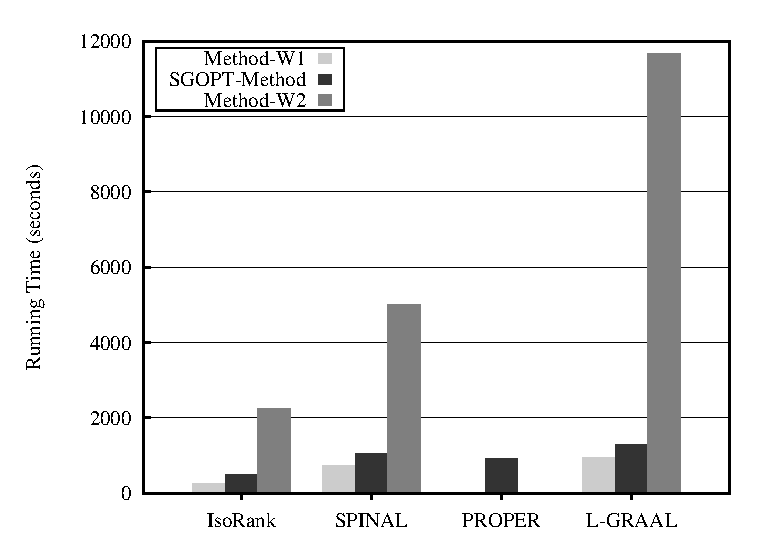
\includegraphics[width=\linewidth]{pic/ce-dm-Time.eps}
            \label{ce-dm-Time}
        \end{minipage}
    }
    \caption{Experiment results using four methods in three ways. Alignments of all three ways are compared using the CE measurement and running time.}
    \label{ce-dm}
\end{figure}

\textbf{The improvement of the SGOPT method}. Fig.~\ref{improveCE} shows the improvement of the CE measurement in all experiments. For IsoRank, the improvement is extreme good. Besides, with three other methods, SGOPT still have about 20\% improvement. In the experiment of hs-sc, we even have a 60\% improvement while running SGOPT-SPINAL. 
\begin{figure}[!htbp]
    \centering
    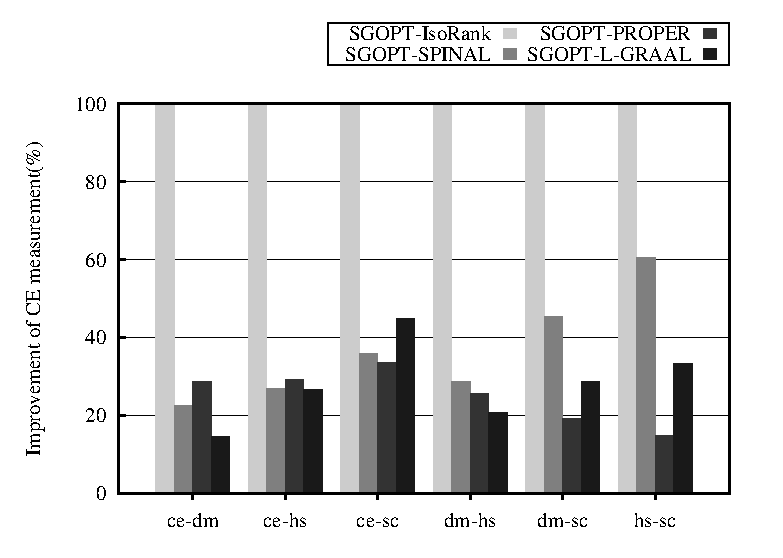
\includegraphics[width=\linewidth]{pic/improveCE.eps}
    \caption{Improvement of the CE measurement while using SGOPT based on alignment produced by different methods. ce-dm is short for aligning C.elegans and D.melanogaster PPI networks, so as the others}
    \label{improveCE}
\end{figure}

%@@@@@@@@@@@@@@@@@@@@@@@@@@@@@@@@@@@@@@@@@@@@@@@@@@@@@@@@@@@@@@
\subsection{Comparison using different measurements}
While SGOPT is a method which aims to improve the CE measurement of the alignment, we also test it on other measurements to see if they can be improved. Fig.~\ref{improveOther} shows the results of improvement of other measurements in all experiments while running SGOPT base on alignments produced by different methods. 

From the aspect of different methods, for the IsoRank and SPINAL method, we observe that SGOPT can improve all the measurements across all the experiments, specifically, the improvement of IsoRank is far more than we expected and the improvement of SPINAL is from 20\% to 60\% for different measurements and experiments. In the experiment of hs-sc, the improvement of SPINAL is the best. For the PROPER and L-GRAAL method, the improvement is not good as IsoRank and SPINAL, and we observe that SGOPT can not improve the DICS and DS$^3$ measurements in the experiments of ce-dm, ce-hs, ce-hs and dm-hs.

From the aspects of different measurements, we find that the improvement of the DEC measurement is the best, and the next is the DTWEC measurement. The DICS and DS$^3$ measurements are the worst. Thus, we conclude that SGOPT is more suitable for aligning PPI networks when the DEC and DTWEC measurements are used.

From the aspects of different experiments, we can see that for the experiments of dm-hs, dm-sc, hs-sc, SGOPT can get better improvements compared to the experiments of ce-dm, ce-hs, ce-sc. We guess that is because SGOPT aims to find more conserved edges, so it has more improvement space when aligning two PPI networks which have large number of edges.
\begin{figure*}[!t]
    \subfigure[The DEC measurement]{
        \begin{minipage}[b]{0.5\linewidth}
            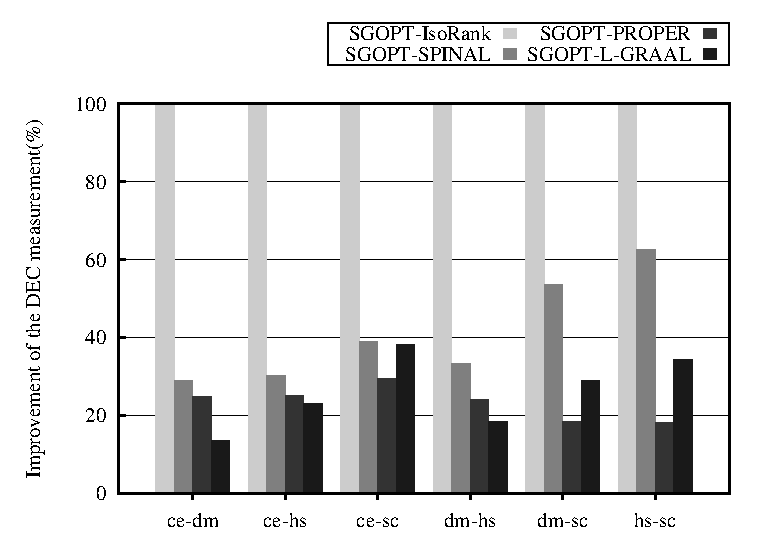
\includegraphics[scale=0.6]{pic/improveDEC.eps}
            \label{improveDEC}
        \end{minipage}
    }
   \subfigure[The DICS measurement]{
        \begin{minipage}[b]{0.5\linewidth}
            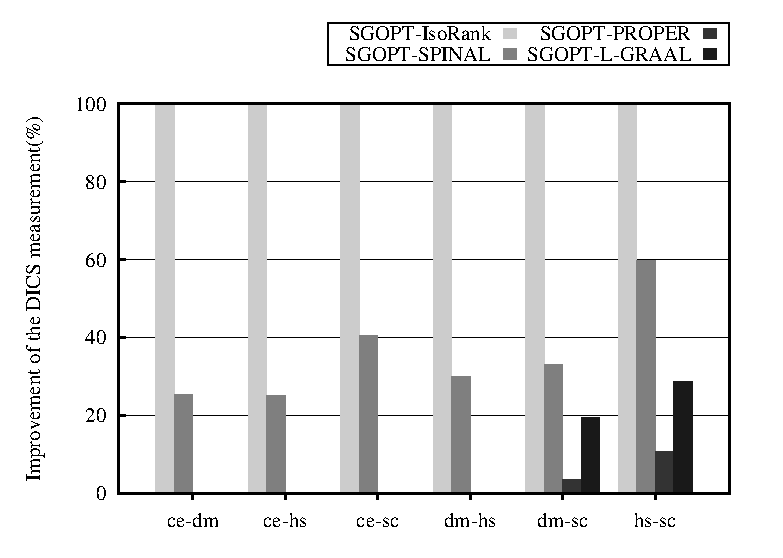
\includegraphics[scale=0.6]{pic/improveDICS.eps}
            \label{improveDICS}
        \end{minipage}
    }
     \subfigure[The DS$^3$ measurement]{
        \begin{minipage}[b]{0.5\linewidth}
            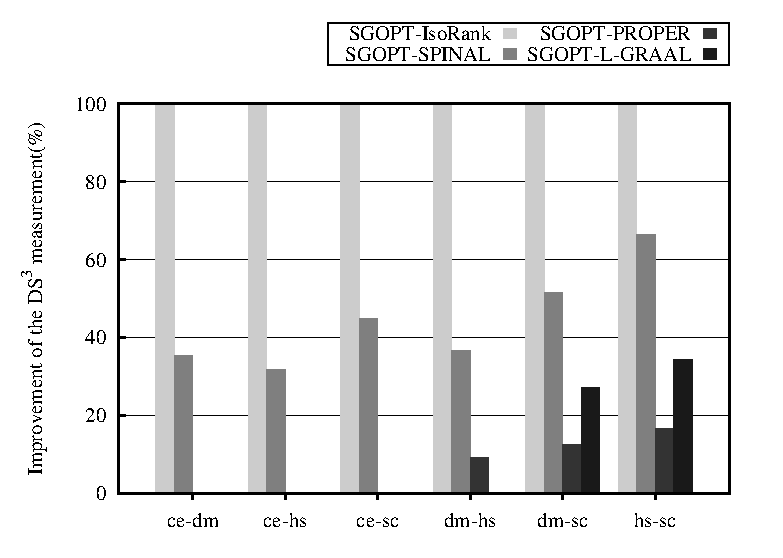
\includegraphics[scale=0.6]{pic/improveDS3.eps}
            \label{improveDS3}
        \end{minipage}
    }
     \subfigure[The DTWEC measurement]{
        \begin{minipage}[b]{0.5\linewidth}
            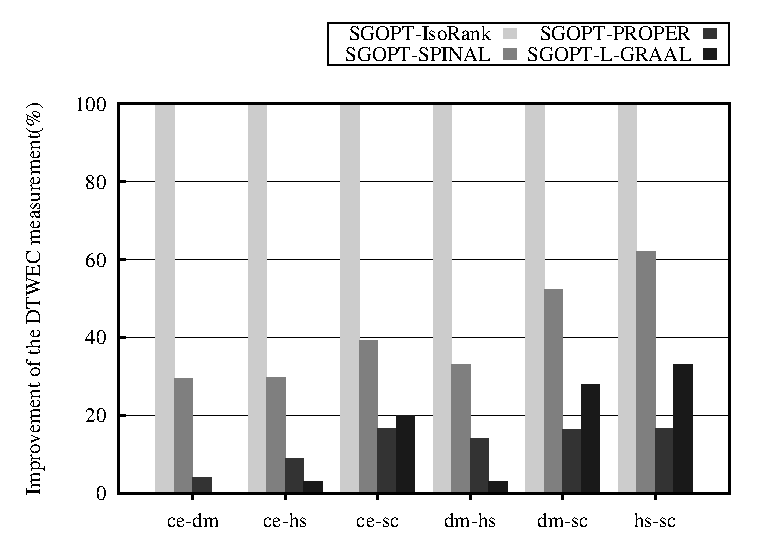
\includegraphics[scale=0.6]{pic/improveDTWEC.eps}
            \label{improveDTWEC}
        \end{minipage}
    }
    \caption{Improvement of the other measurements while using SGOPT base on alignments produced by different methods.}
    \label{improveOther}
\end{figure*}

%@@@@@@@@@@@@@@@@@@@@@@@@@@@@@@@@@@@@@@@@@@@@@@@@@@@@@@@@@@@@@@@
\section{Conclusion}
In this paper, we focus on the alignment of dynamic PPI networks which could be a new topic. And we present our framework SGOPT for transforming static alignments to dynamic alignments. We show that SGOPT could be an efficient time-saving framework to improve the quality of any alignments produced by state-of-the-art static alignment methods. While dynamic PPI networks get more and more attentions nowadays, SGOPT could be a first attempt to solving the problem of aligning dynamic PPI networks.
%\begin{enumerate}
%\item this is item, use enumerate
%\item this is item, use enumerate
%\item this is item, use enumerate
%\end{enumerate}



\section*{Acknowledgements}
\section*{Funding}

\bibliographystyle{natbib}
\bibliography{document}

\end{document}
